\documentclass[12pt,a4paper]{report}

%Image-related packages
\usepackage{graphicx}
\usepackage{subcaption}
\usepackage[export]{adjustbox}

%Style
\setlength{\parskip}{1em plus 0.25em minus 0.25em}
\renewcommand{\baselinestretch}{1.5}

%Table of contents, figures, tables
\usepackage[nottoc]{tocbibind}

\usepackage{hyperref}
\usepackage{xcolor}
\hypersetup{
    colorlinks,
    linkcolor={blue!50!black},
    citecolor={blue!50!black},
    urlcolor={blue!80!black}
}

\usepackage{cite}
\usepackage{chemformula}
\usepackage{appendix}

%Table style
\usepackage{multirow}
\usepackage{tabularx}
\setlength{\arrayrulewidth}{0.2mm} %The thickness of the borders
\setlength{\tabcolsep}{18pt} %The space between the text and the left/right border
\renewcommand{\arraystretch}{1.5} %The height of each row
\usepackage{colortbl} %Table cell colour

%Header & footer
\usepackage{fancyhdr}

%Redefines the /today command
\renewcommand{\today}{\ifcase \month \or January\or February\or March\or April\or May%
\or June\or July\or August\or September\or October\or November\or December\fi\:%
\number \year}

%Glossary
\usepackage{glossaries}
\makeglossaries

\newglossaryentry{ghg}
{
    name=GHG,
    description={Greenhouse gas}
}

\newglossaryentry{co2}
{
    name=\ch{CO2},
    description={Carbon dioxide}
}

\newglossaryentry{eu}
{
    name=EU,
    description={European Union}
}

\newglossaryentry{pv}
{
    name=PV,
    description={Photovoltaic}
}

\newglossaryentry{ee}
{
    name=EE,
    description={Energy efficiency}
}

\newglossaryentry{sd}
{
    name=SD,
    description={Sustainabe Development}
}

\newglossaryentry{re}
{
    name=RE,
    description={Renewable energy}
}

\newglossaryentry{sems}
{
    name=SEMS,
    description={Smart energy management system}
}

\newglossaryentry{nape}
{
    name=NAPE,
    description={The National Action Plan on Energy Efficiency}
}

\newglossaryentry{dr}
{
    name=DR,
    description={Demand response}
}

\newglossaryentry{hp}
{
    name=HP,
    description={Heat pump}
}

\newglossaryentry{rs}
{
    name=RS,
    description={Recommender systems}
}

\newglossaryentry{nl}
{
    name=NL,
    description={Natural language}
}

\newglossaryentry{iv}
{
    name=IV,
    description={Information Visualisation}
}

\begin{document}

\begin{titlepage}

\begin{center}

\vspace*{-1cm}

\begin{figure}[h]
  \begin{subfigure}{0.50\textwidth}
    
\includegraphics[width=0.8\linewidth, left]{Images/siegen.png}
  \end{subfigure}
  \begin{subfigure}{0.49\textwidth}
    
\includegraphics[width=0.8\linewidth, right]{Images/isi.jpeg}
  \end{subfigure}
\end{figure}

\vfill

%\textbf{\large Research Proposal}\\[10pt]
{\Large \bf Filling the Information Gap of House Owners and Technologies: A Design Case Study of a smart recommender for home energy system} \\

\vfill
In partial fulfilment of the requirement for the degree of\\
{\large \bf MASTER OF SCIENCE}\\
in\\ 
{\large \bf Human Computer Interaction } \\
{\em by} \\
{\large \bf Yanwei Miao} \\
{\large \bf (1627738)}\\

Under the supervision of \\
{\bf \large Prof. Dr. Gunnar Stevens} \\
{\bf \large Dr. Songmin Yu} \\

\vfill

{\it \large \today}

\end{center}

\end{titlepage}

\clearpage
\pagenumbering{roman} \setcounter{page}{2}
\begin{center}
{\Large{\bf{ABSTRACT}}}
\end{center}

\noindent

Climate change is a threat to the environment and society. 
Evidences show human behaviours are the main contributions to the global warming. 
There is an ergent need to slow down the process of global warming. 
The goal has been raised in the Paris Agreement.
And at the EU level, there are 2 goals that should be achieved by 2030 and 2050.  

\clearpage
\tableofcontents
\clearpage
\listoffigures
\listoftables

\newpage
\clearpage % Start a new page

\noindent

{\Huge{\bf{Notations and Abbreviations}}}\
\\[6pt] 

\newglossaryentry{ghg}
{
    name=GHG,
    description={greenhouse gas}
}

\newglossaryentry{co2}
{
    name=\ch{CO2},
    description={carbon dioxide}
}

\newglossaryentry{eu}
{
    name=EU,
    description={European Union}
}

\printglossaries

\newpage

\pagenumbering{arabic}
\setcounter{page}{1}

\chapter{Introduction}

Human-induced climate change is causing dangerous and widespread disruption in nature, thereby affecting billions of lives globally. \cite{ipcc}. 
To tackle climate change and its negative impacts, two main strategies are addressed: climate change mitigation and adaptation.

\begin{itemize}
  \item \textbf{Climate change mitigation} refers to the actions taken to reduce or prevent greenhouse gas (\gls{ghg}) emissions and ultimately stabilize the concentration of these gases in the atmosphere to limit global warming and its adverse effects \cite{handbook}.
  This goal entails a range of related projects, spanning farming, land use, peatland management, renewable energies, and energy efficiency. Integrated projects that implement climate change mitigation strategies and action plans at regional or national levels are also pertinent \cite{ec}.
  Notably, to curb carbon dioxide (\gls{co2}) emissions in the energy system, two main approaches are pursued:
\emph{
  (1) reducing energy consumption on the demand side through efficiency improvement and behavioral changes and
  (2) transitioning to renewable energy sources on the supply side.
}
%These terms go hand-in-hand as we tackle the climate crisis.
  \item \textbf{Climate change adaptation} encompasses measures to manage the adverse impacts of climate change, such as natural disasters, changes in precipitation patterns, and rising sea levels, among others \cite{handbook},
  which includes projects relating to urban adaptation and land-use planning, infrastructure resilience, sustainable water management in drought-prone areas, flood and coastal management, as well as the resilience of the agricultural, forestry, and tourism sectors \cite{ec}.  
\end{itemize}

The work in this thesis belongs to the category of climate change mitigation. 
%Following the work in the newTRENDs project\footnote{https://newtrends2020.eu/}, 
%we look at how the impact of ``new societal trends'' on the future development of the energy demand.
%Then, we apply the HCI techniques in designing a tool to guide decisions on household's investments in energy efficiency and renewables from a techno-economic perspective.  %the basic motivation of this thesis in one sentence.
%Climate change can only be tackled if people actively engage, as consumers and as citizens \cite{clean}.


\section{Mitigating Climate Change through Energy Transition}
The Paris Agreement, a historic international agreement, sets long-term goals to substantially reduce global emissions and limit the global temperature increase to 2 degrees Celsius in this century \cite{paris}.
To achieve this ambitious goal, the world is facing an unprecedented imperative to a rapid transition in the energy sector. 
The European Union (\gls{eu})'s "Energy 2020. A strategy for competitive, sustainable and secure energy" and "Energy Roadmap 2050" are key strategy papers guiding energy developments in the \gls{eu} \cite{roadmap}, aiming to lead in global climate action and achieve net-zero emissions by 2050 through a socially-fair and cost-efficient transition \cite{clean}. 


\section{Households in energy transition}

Households are a crucial component of the energy transition, as they are responsible for a significant proportion of final energy consumption in the \gls{eu}, as highlighted by Eurostat's 2023 report. 
In fact, in 2020, the residential sector accounted for 27.4\% of total final energy consumption or 18.7\% of gross inland energy consumption in the \gls{eu} \cite{eurostat}. 
Therefore, reducing energy consumption in households through energy-efficient building construction and renovations, as well as digitalisation and smart demand-side management, can have a significant impact on achieving the \gls{eu}'s energy and climate targets \cite{building}. 
This underscores the importance of developing and implementing effective policies and strategies to promote energy efficiency and renewable energy use in households to facilitate the energy transition.


\section{Technologies for home energy system}

Technologies for home energy systems have rapidly advanced in recent years, with a growing focus on energy efficiency and renewable energy sources. 
Smart home technologies, such as energy management systems, allow households to optimise their energy consumption and reduce waste. 
Moreover, rooftop solar panels and home battery storage systems enable households to generate and store their own renewable energy, reducing dependence on the grid and lowering electricity bills. 
In addition, the integration of electric vehicles with home energy systems can further reduce household carbon emissions and provide a source of backup power. 
These technologies have the potential to significantly transform the way households consume and generate energy, contributing to a more sustainable and resilient energy system.


\section{Research gaps}

Despite the growing availability and accessibility of home energy technologies, there remains a significant information gap regarding their effective utilisation. 
Government policies aimed at promoting the adoption of these technologies have resulted in an infrastructure that supports the use of electricity and lowers the costs of using renewable energy. 
However, a survey conducted by Palmer et al. identified a lack of knowledge and guidance among homeowners, preventing them from maximising the benefits of these investments in terms of reducing future energy expenses \cite{informationgap}. 
As a result, there is a research gap in exploring effective ways to educate and inform house owners on the utilisation of home energy technologies. 


\section{Research questions and aims}

The following research questions will guide this study: 
\begin{enumerate}
  \item How can HCI help fill the information gap in households' knowledge of energy technology and support decision-making on the adoption of clean energy and energy-efficient technologies?
  \item Is the information making a difference? 
\end{enumerate}
The aim of this study is to address the information gap and support homeowners in their decision-making process regarding the adoption of clean energy and energy-efficient technologies. 
The study also seeks to evaluate the effectiveness of such a nudging approach. 

The following research objectives will aid in answering the research questions: 
\begin{itemize}
  \item Conduct a thorough review of relevant literature to identify existing gaps and opportunities in the field. 
  \item Develop a user-friendly and accessible interface for providing information about energy-efficient technologies and their benefits to households.
  \item Design and implement interactive tools that enable households to estimate the costs and benefits of adopting different energy-efficient technologies and renewable energy sources.
  \item Conduct user studies to evaluate the impact of the developed interventions on households' thoughts of energy-efficient technologies and renewable energy sources, using both quantitative and qualitative methods.
  \item Analyse the data collected from the user studies to gain insights into the users' needs and preferences, as well as the effectiveness of the interventions.
  \item Write the thesis that presents the findings, conclusions and recommendations based on the research conducted. 
%  \item Investigating the data required by the FLEX-Operation model. 
%  \item Identifying the typical European household types and understanding their perceptions of the household energy system. 
%  \item Providing recommendations and evaluations of the technological performance and economic feasibility of household's energy system.
%  \item Designing the web application with user-centred approaches. 
%  \item Using data visualisation techniques to ensure explainability of the recommendations. 
%  \item Developing the frontend and backend web application. 
%  \item Evaluating the explainability of the recommendations from users' perspectives and measuring the impact of the households‘ perceptions towards proposed solutions. 
%  \item Allowing long-term event tracking for design iteration. 
\end{itemize}

%Meanwhile, the following criteria should be taken into consideration 
%while building a software application from a user's perspective: 

%\begin{itemize}
%  \item The software should be easy and effortless to use. 
%  \item The interactions should be intuiative. 
%  \item The assessments should be clear explained to users. 
%\end{itemize}

%Accordingly, three subquestions are raised: 
%\begin{enumerate}
%  \item What are the data required by the FLEX-Operation model from households? 
%  \item What are the typical European household profiles? 
%  \item How to offer trustworthy and user-friendly recommendations to European households from a techno-economic perspective? 
%\end{enumerate}

This thesis aims to contribute to the HCI community by exploring the use of technology to fill the information gap in households' knowledge of energy technology and support decision-making on the adoption of clean energy and energy-efficient technologies. 
It will offer insights into the design and development of personalised and professional home energy system recommendations and their effectiveness in promoting the adoption of those technologies. 
The study will also provide insights into the user experience of the intervention and how it can be further improved to support sustainable energy choices. 
Overall, this thesis seeks to advance the understanding of the role of technology in promoting sustainable energy consumption in households, and its findings can inform the development of future HCI interventions to address environmental challenges. 


\section{Justification and planning} 

\subsection{Justification}

The proposed thesis project will combine research and application aspects, 
which is important because it will allow for a comprehensive understanding of the topic being studied. 
Conducting a thorough literature review will provide a strong foundation for the research, 
while the development of software applications will allow for practical implementation of the findings. 
In addition, interviews with industry professionals and stakeholders will provide valuable insights into the real-world challenges and opportunities in the field. 
Finally, the evaluation process will involve much data analysis, enabling the research to draw valid and reliable conclusions. 
Thus, the proposed thesis project will contribute to a well-rounded and informative study, and is believed to be justified for 30 credits.


\subsection{Supervision}

This master thesis project will be supervised by 
Prof. Dr. Gunnar Stevens (\href{mailto:gunnar.stevens@uni-siegen.de}{gunnar.stevens@uni-siegen.de}) at Siegen University and 
Dr. Songming Yu (\href{mailto:songmin.yu@isi.fraunhofer.de}{songmin.yu@isi.fraunhofer.de}) from The Fraunhofer Institute for Systems and Innovation Research. 


\subsection{Time planning}

The following is the time allocation for the research objectives, which are scheduled to be completed in 26 weeks. \\

\begin{table}[h]
  \begin{center}
    \begin{tabular}{ p{.05\textwidth} p{.80\textwidth} }
      \cellcolor[rgb]{0.94,0.96,0.98}1 & Literature review \\
      \cellcolor[rgb]{0.86,0.90,0.96}2 & Design interfaces\\ 
      \cellcolor[rgb]{0.78,0.84,0.94}3 & Develope the software tool\\
      \cellcolor[rgb]{0.71,0.78,0.92}4 & User studies \\
      \cellcolor[rgb]{0.63,0.73,0.89}5 & Analyse data\\
      \cellcolor[rgb]{0.55,0.67,0.87}6 & Write thesis \\
    \end{tabular}
    \caption{Research objectives}
    \label{tab:objectives}
  \end{center}
\end{table}

\begin{table}[h]
  \begin{center}
    \addtolength{\tabcolsep}{4pt} % new width
    \renewcommand{\arraystretch}{0.8} % new height
      \begin{tabular}{ l c c c c c c c }
        && \textbf{1} & \textbf{2} & \textbf{3} & \textbf{4} & \textbf{5} & \textbf{6} \\ 
        \multirow{4}{*}{\textbf{Feb}} & w1 & \cellcolor[rgb]{0.94,0.96,0.98} \\ & w2 & \cellcolor[rgb]{0.94,0.96,0.98} \\ & w3 & \cellcolor[rgb]{0.94,0.96,0.98} \\ & w4 & \cellcolor[rgb]{0.94,0.96,0.98} \\ 
        \multirow{5}{*}{\textbf{Mar}} & w5 && \cellcolor[rgb]{0.86,0.90,0.96} \\ & w6 && \cellcolor[rgb]{0.86,0.90,0.96} \\ & w7 && \cellcolor[rgb]{0.86,0.90,0.96} \\ & w8 && \cellcolor[rgb]{0.86,0.90,0.96} \\ & w9 && \cellcolor[rgb]{0.86,0.90,0.96} \\ 
        \multirow{4}{*}{\textbf{Apr}} & w10 &&& \cellcolor[rgb]{0.78,0.84,0.94} \\ & w11 &&& \cellcolor[rgb]{0.78,0.84,0.94} \\ & w12 &&& \cellcolor[rgb]{0.78,0.84,0.94} \\ & w13 &&& \cellcolor[rgb]{0.78,0.84,0.94} \\ 
        \multirow{4}{*}{\textbf{May}} & w14 &&&& \cellcolor[rgb]{0.71,0.78,0.92} \\ & w15 &&&& \cellcolor[rgb]{0.71,0.78,0.92} \\ & w16 &&&& \cellcolor[rgb]{0.71,0.78,0.92} \\ & w17 &&&& \cellcolor[rgb]{0.71,0.78,0.92} \\ 
        \multirow{5}{*}{\textbf{Jun}} & w18 &&&&& \cellcolor[rgb]{0.63,0.73,0.89} \\ & w19 &&&&& \cellcolor[rgb]{0.63,0.73,0.89} \\ & w20 &&&&& \cellcolor[rgb]{0.63,0.73,0.89} \\ & w21 &&&&& \cellcolor[rgb]{0.63,0.73,0.89} \\ & w22 &&&&& \cellcolor[rgb]{0.63,0.73,0.89} \\ 
        \multirow{4}{*}{\textbf{Jul}} & w23 &&&&&& \cellcolor[rgb]{0.55,0.67,0.87} \\ & w24 &&&&&& \cellcolor[rgb]{0.55,0.67,0.87} \\ & w25 &&&&&& \cellcolor[rgb]{0.55,0.67,0.87} \\ & w26 &&&&&& \cellcolor[rgb]{0.55,0.67,0.87} \\ 
      \end{tabular}
    \caption{Time planning}
    \label{tab:planning}
  \end{center}
\end{table}
\chapter{The newTRENDs Project} 

The aim of NewTRENDs is to increase the qualitative and quantitative understanding of impacts of New Societal Trends on energy consumption and to improve the modelling of energy demand, energy efficiency and policy instruments \cite{fraunhofer}. 

\section{Concept}

%The newTRENDs project develops the analytical basis for a ``2050 Energy Efficiency Vision" by considering New Societal Trends in energy demand modeling \cite{newtrends}.

With increasing renewable generation integrated into the power system, supply-side fluctuations must be balanced by demand-side flexibility. 
Electrification and demand response (DR) are becoming increasingly relevant to the heating transition of buildings, which demands the diffusion of

\begin{itemize}
  \item heat pumps (HPs),
  \item photovoltaic (PV) and energy storage (e.g., battery and hot water tank),
  \item smart energy management systems (SEMSs).
\end{itemize}

Combining the three technologies is also beneficial from an individual household (or building) perspective. The household can optimize the heat pump operation to reduce energy costs by saving energy in the tanks or pre-heat the building when the electricity price is lower. Besides, the energy-saving benefit could be further increased with PV and battery system.
From a market perspective, DR flexibility and PV generation also facilitate the concept of "energy community". The households can trade electricity with each other (peer-to-peer, P2P) within a local micro-grid or even trade with the other side of the country through the national grid, depending on the infrastructure, business model, and policies. In addition, households can also buy the services from an "aggregator", who bundles and manages the flexibility of small consumers and producers and participate in the market activities (Kerscher and Arboleya 2022). 
Promoted by the declining costs of technologies and support policies, more and more household "consumers" are expected to become "prosumers" (with PV) and "prosumagers" (plus energy storage and SEMS) (Fereidoon Sioshansi 2019).

\section{FLEX models}

The FLEX-Operation and FLEX-Community models were built to improve the building modeling suite and to analyze the societal trends of prosumaging and energy communities.
The figure \ref{fig:flex} shows how FLEX interacts with other bottom-up models involved in the newTRENDs project.

\begin{figure}[h]
  \centering
  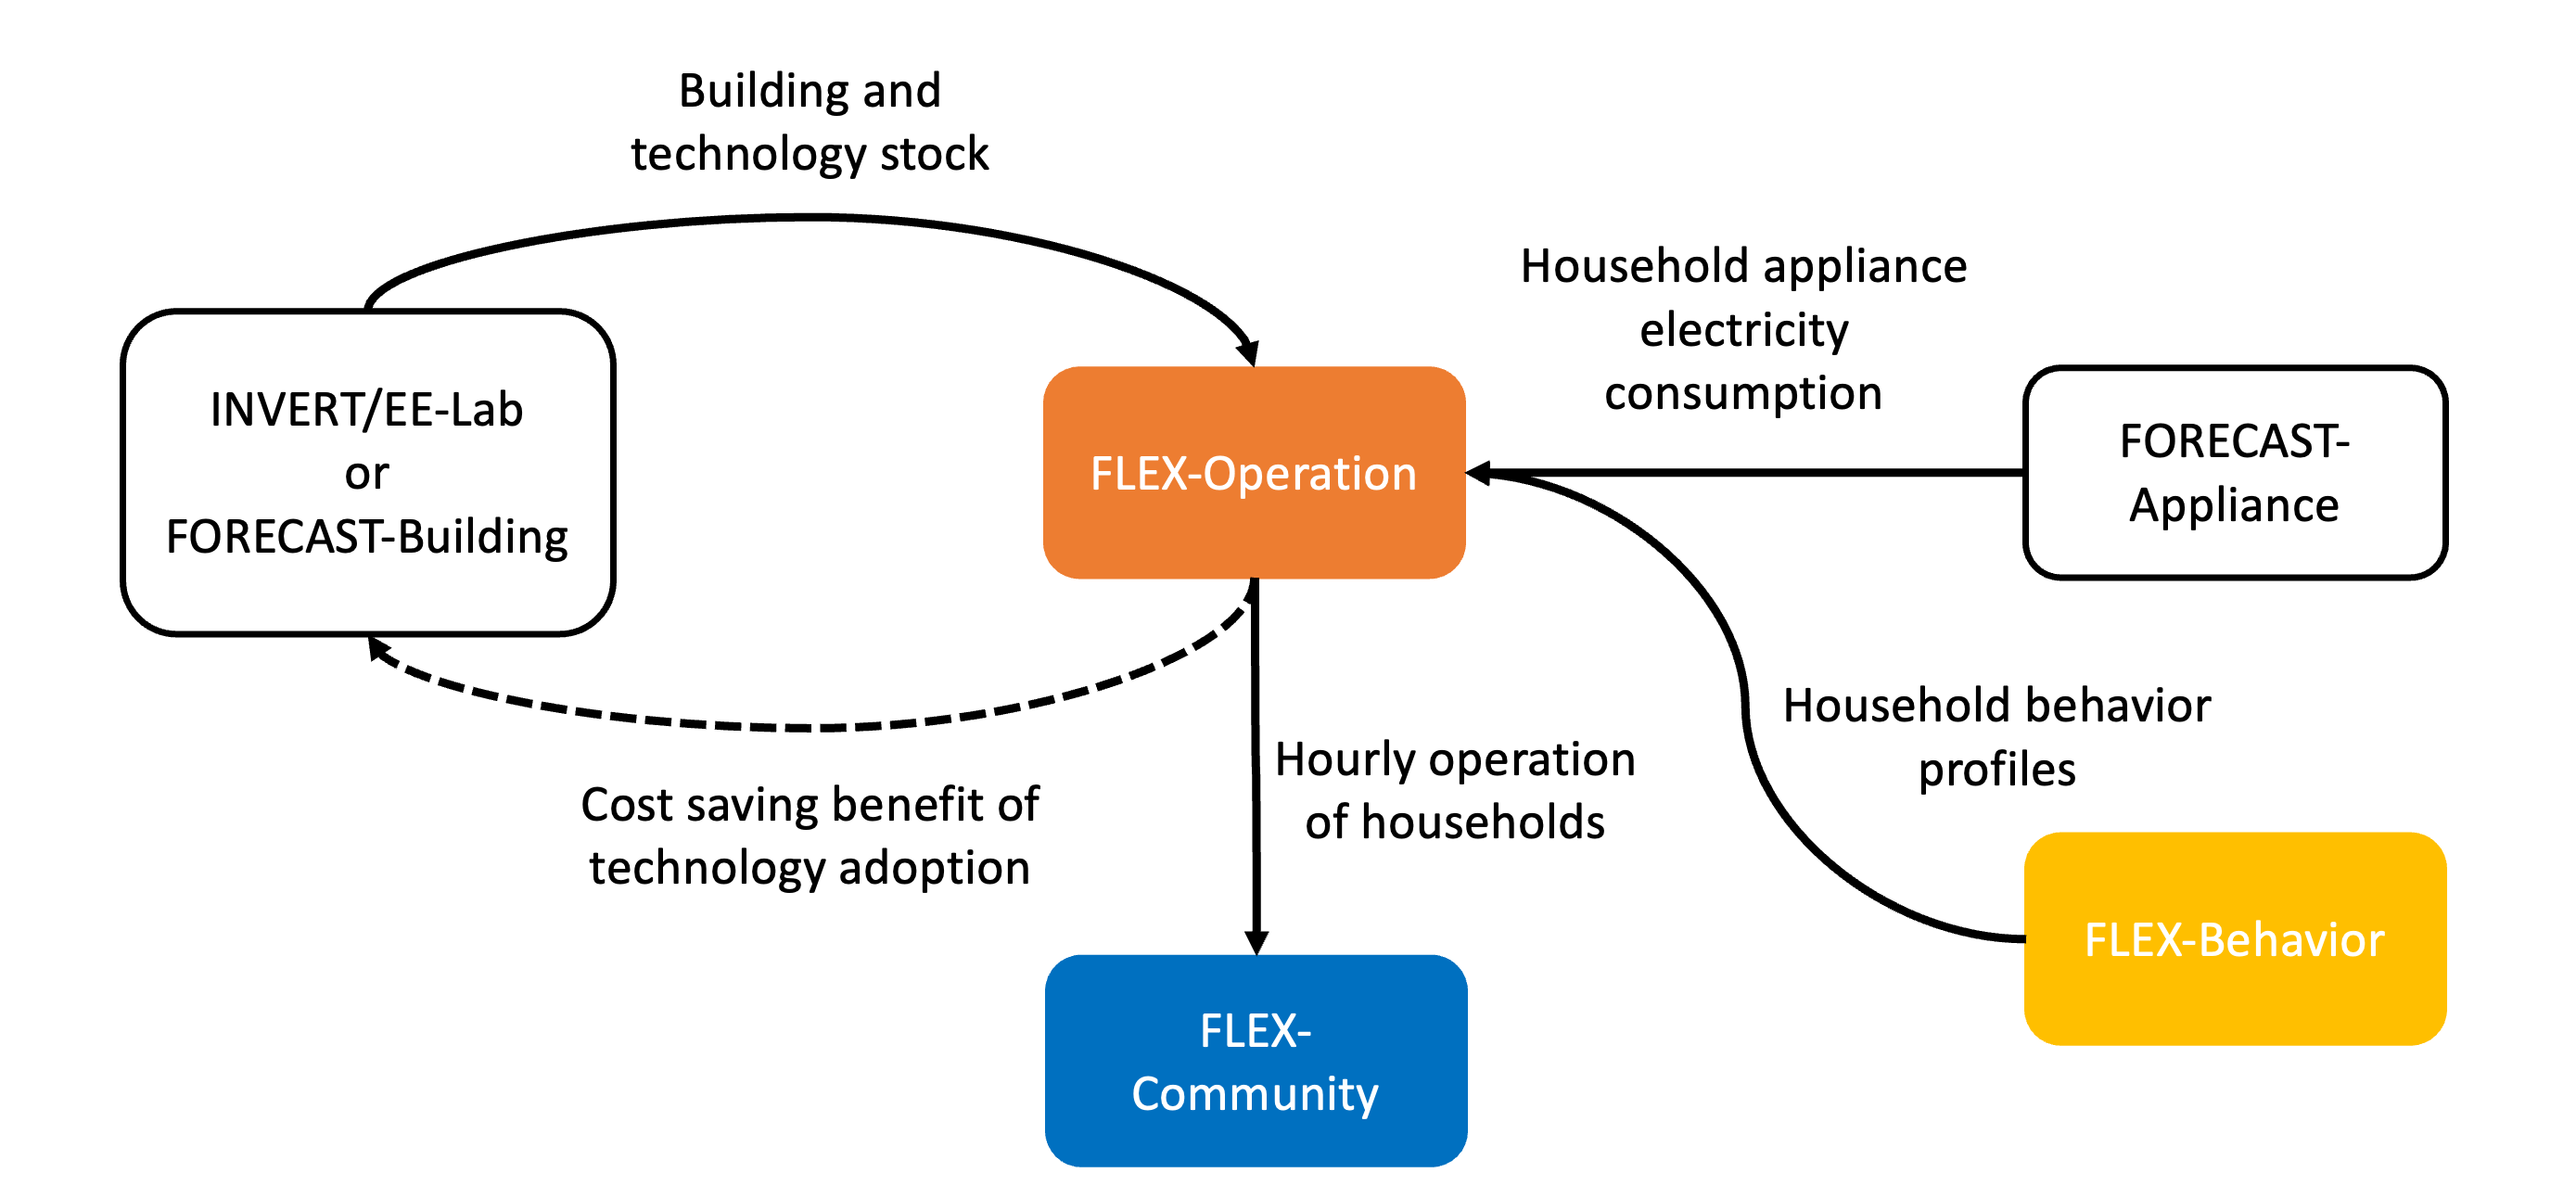
\includegraphics[width=\textwidth]{Images/flex.png}
  \caption{FLEX modeling suite}
  \label{fig:flex}
\end{figure}

INVERT/EE-Lab and FORECAST-Appliance are the two models that can cover the energy consumption of residential buildings. The two models complement each other and cover the total energy consumption of households. 
However, both INVERT/EE-Lab and FORECAST-Appliance calculate the energy consumption at the annual resolution and cannot model the prosumaging behavior and energy community, which requires an hourly resolution to consider the impact of household behavior, PV generation, and energy storage (thermal and battery) on energy consumption. In this regard, we developed the FLEX- Operation and FLEX-Community models to improve the building modeling suite and support relevant policy analysis.

\subsection{FLEX-Community}

FLEX-Community models the operation of an energy community, i.e., household interaction, aggregator optimisation. 
It can be applied to support the aggregators designing and evaluating business models, as well as making investment decisions, for example, the self-owned battery, PV panels, etc.

\subsection{FLEX-Behavior}

FLEX-Behavior models the behavior (activity profile) of households' and corresponding load profiles. 
It generates the hourly activity and energy demand profile of a pre-defined individual household. 
The results include

\begin{enumerate}
  \item appliance electricity demand,
  \item domestic hot water demand,
  \item driving profile, and
  \item building occupation.
\end{enumerate}

\subsection{FLEX-Operation}

FLEX-Operation models the energy system operation of an individual household in hourly resolution.  
It calculates the energy consumption of each representative building, including operation of technologies (e.g., battery, PV, heat pump, etc.) and load profiles in hourly resolution.

Data is considered by the model

\begin{itemize}
  \item building,
  \item heating system (heat pump, fuel-based boiler, electric heater),
  \item thermal storages for space heating and domestic hot water,
  \item space cooling technology,
  \item PV,
  \item battery, and
  \item electric vehicle.
\end{itemize}

\section{Motivations}

As a part of the newTRENDs project, 
the proposed thesis will focus solely on the implementation of the FLEX-Operation model.  
By employing the model to 
suggest reliable, cost-effective energy optimisation solutions 
while giving households with comparable predicted statistics on their energy consumption for the time frame. 
Despite the fact that the model primarily responds to societal trends for 2030, 
which means it provides more flexible suggestions when a household already owns a photovoltaic (\gls{pv}) system, 
this could be as well an opportunity to nudge the European households who currently rely on other energy resources
to switch to renewable energy when feasible. 
And it will be beneficial not only to the environment but also to consumers. 

\section{Research gaps and questions}

There is a lack of case study research of promoting energy optimisation solutions. 
The aim of this proposed thesis is to design and develop a user-friendly web application for an energy optimisation recommendation system.

The following criteria should be taken into account while building a user-friendly application: 

\begin{itemize}
  \item It should be easy and effortless for using. 
  \item The interactions should be intuiative. 
  \item The recommandations should be clear explained. 
\end{itemize}

Projectives: 

\begin{itemize}
  \item implementation of proposed smart energy optimisation recommender as a web application, using data visualisation techniques designed for different types of households. 
  \item evaluation of the explainability of smart energy optimisation recommender at the user level and measuring the impact of the households perceptions towards energy optimisation solutions. 
  \item provide a design guideline on how to enable trust in energy optimisation solutions when trying to promote green energy plans. 
\end{itemize}

Resaerch questions:

\begin{itemize}
  \item How are typical European household profiles?
  \item How to simplify the user information obtain process with the decision tree technique?
  \item How to suggest explainable energy optimisation solutions?
\end{itemize}


\chapter{Methodology} 

The study uses Design Case Studies \cite{dcs} as the research framework. 

In the pre-study phase, 
the primary focus was to investigate existing practices and tools that can aid homeowners in gaining knowledge about renewable energy and energy-efficient technologies, as well as their benefits. 
To achieve this, we conducted searches online and reviewed relevant literature to gather information. 
As there were limited successful initiatives available in the market, we identified two related options: energy audits and research models. 
We studied both options to identify effective methods that can support homeowners in understanding renewable energy and energy-efficient technologies, along with their associated benefits.

Following the pre-study, 
we recognised a suitable approach aligned with the learning theory, 
and developed an innovative design concept: a personalised home energy system recommender.
To ensure its effectiveness, 
we started by investigating homeowners' motivations for investing in energy technologies through literature. 
Next, our focus was on providing recommendations that are aligned with user needs, 
and we placed great emphasis on enhancing the explainability of the system.

Furthermore, during the IT artefact design process, 
multiple factors were taken into account, including usability, user experience, and the chosen medium. 
Additionally, 5 formative evaluations were conducted on high-fidelity wireframes, 
which helped identify some issues that were then addressed through design iterations. 

After the service was programmed and made available online, 
we conducted a summative investigation to assess the appropriation of the artefact,
with a specific focus on two aspects:
\begin{enumerate}
    \item Do users enhance their knowledge about energy technologies and the advantages of their adoption through the service?
    \item Do users have trust in the recommendations provided by the system?
\end{enumerate}
6 qualitative evaluations were performed with 7 actual house owners. 
These evaluations were conducted through semi-structured interviews, 
each lasting approximately one to three hours. 

After conducting the evaluations, a thematic analysis was performed to gain deeper insights into users' experiences and perceptions. 
This analysis provided valuable feedback and insights that can be used for the next design iteration, allowing for further improvements and enhancements to the artefact. 

%The methodology adopted in this study is based on the Design Case Studies framework. 
%The pre-study phase will begin by conducting a comprehensive review of the literature to identify best practices for providing households with personalised and professional home energy system recommendations, as well as techno-economic assessments.
%Based on the findings from the pre-study, I will then design the interfaces of the intervention. 
%The interfaces will be developed to provide an intuitive and user-friendly experience that can easily be understood by households. 
%Following the development phase, real users will be invited to use the intervention, and feedback will be collected both qualitatively and quantitatively. 
%The qualitative data will be collected through interviews with participants, while the quantitative data will be collected through surveys. 
%Finally, the collected data will be analysed to evaluate households thoughts about the recommendations and energy technologies. 
%The entire process will be documented and reported in the form of a thesis. 
\chapter{Supervision agreements and time planning} 

Introductory lines...

\section{Justification for 30 ECTS}

Research + design + develop

\section{Supervision}

This master thesis project will be supervised by 
Prof. Dr. Gunnar Stevens (Gunnar.Stevens@uni-siegen.de) and 
Dr. Songming Yu (songmin.yu@isi.fraunhofer.de).  

\section{Time planning}

Text here...

\appendix

\appendixpage
\addappheadtotoc
\chapter{Input of the FLEX models}
\label{appendix:inputdata}

\begin{center}
    \small
    \begin{longtable}{ | p{.10\textwidth} | p{.80\textwidth} | }
        \hline 
        \multicolumn{1}{|c|}{\textbf{Category}} & \multicolumn{1}{c|}{\textbf{Data}} \\ 
        \hline 
        \endfirsthead

        \multicolumn{2}{l}
        {{\bfseries \tablename\ \thetable{} -- continued from previous page}} \\
        \hline \multicolumn{1}{|c|}{\textbf{Category}} &
        \multicolumn{1}{c|}{\textbf{Data}} \\  
        \endhead

        \multicolumn{2}{|r|}{{Continued on next page}} \\ 
        \hline
        \endfoot

        \endlastfoot
            Behaviour profile & id\_hour, people\_at\_home\_profile\_1, hot\_water\_demand\_profile\_1, appliance\_electricity\_demand\_profile\_1, vehicle\_at\_home\_profile\_1, vehicle\_distance\_profile\_1. \\
            \hline 
            Battery & ID\_Battery, capacity, capacity\_unit, charge\_efficiency, charge\_power\_max, charge\_power\_max\_unit, discharge\_efficiency, discharge\_power\_max, discharge\_power\_max\_unit. \\
            \hline 
            Behaviour & ID\_Behavior, id\_people\_at\_home\_profile, target\_temperature\_at\_home\_max, target\_temperature\_at\_home\_min, target\_temperature\_not\_at\_home\_max, target\_temperature\_not\_at\_home\_min, shading\_solar\_reduction\_rate, shading\_threshold\_temperature, temperature\_unit, id\_hot\_water\_demand\_profile, hot\_water\_demand\_annual, hot\_water\_demand\_unit, id\_appliance\_electricity\_demand\_profile, appliance\_electricity\_demand\_annual, appliance\_electricity\_demand\_unit, id\_vehicle\_at\_home\_profile, id\_vehicle\_distance\_profile. \\
            \hline 
            Boiler & ID\_Boiler, type, power\_max, power\_max\_unit, carnot\_efficiency\_factor. \\
            \hline 
            Building & ID\_Building, type, construction\_period\_start, construction\_period\_end, person\_num, Af, Hop, Htr\_w, Hve, CM\_factor, Am\_factor, internal\_gains, effective\_window\_area\_west\_east, effective\_window\_area\_south, effective\_window\_area\_north, grid\_power\_max, supply\_temperature. \\
            \hline
            Energy price & ID\_EnergyPrice, id\_electricity, id\_electricity\_feed\_in, id\_gases, price\_unit. \\
            \hline
            Heating element & ID\_HeatingElement, power, power\_unit, efficiency. \\
            \hline 
            Hot water tank & ID\_HotWaterTank, size, size\_unit, surface\_area, surface\_area\_unit, loss, loss\_unit, temperature\_start, temperature\_max, temperature\_min, temperature\_surrounding, temperature\_unit. \\
            \hline 
            \gls{pv} & ID\_PV, size, size\_unit. \\
            \hline
            Region & ID\_Region, code, year, norm\_outside\_temperature. \\
            \hline 
            Space cooling technology & ID\_SpaceCoolingTechnology, efficiency, power, power\_unit. \\
            \hline 
            Space heating tank & ID\_SpaceHeatingTank, size, size\_unit, surface\_area, surface\_area\_unit, loss, loss\_unit, temperature\_start, temperature\_max, temperature\_min, temperature\_surrounding, temperature\_unit. \\
            \hline 
            Vehicle & ID\_Vehicle, type, capacity, capacity\_unit, consumption\_rate, consumption\_rate\_unit, charge\_efficiency, charge\_power\_max, charge\_power\_max\_unit, discharge\_efficiency, discharge\_power\_max, discharge\_power\_max\_unit, charge\_bidirectional. \\
            \hline 
            Energy price & Region, year, id\_hour, electricity\_1, electricity\_2, electricity\_feed\_in\_1, gases\_1. \\
            \hline 
            Region weather & region, year, id\_hour, pv\_generation, pv\_generation\_unit, temperature, temperature\_unit, radiation\_south, radiation\_east, radiation\_west, radiation\_north, radiation\_unit. \\
            \hline 
        \caption{Input data of the FLEX-Operation model}
        \label{tab:inputdata}
    \end{longtable}
\end{center}

\nocite{*} % Without this, only cited materials are displayed in the bibliography.

\bibliographystyle{apalike}
\bibliography{ref}

\end{document}
